\paragraph{Gender Bias in Wikidata}
Gender bias analysis in Wikidata will be performed on 10 Wikidata classes: computer scientist, American singer, American actress/actor, badminton player, businessperson, lawyer, American politician, American writer, American researcher, and American journalist.

To analyze the bias, the first aspect that will be considered is the proportion of each gender in every class. We assume that there are equal numbers of males and females in real-world and this will be the basis to determine if there is any bias in the data. Pearson's chi-square test (goodness-of-fit) is then performed to test the null and alternative hypotheses with significance level of \(\alpha=5\%\) as follows:

\(H_0\): The proportions of males and females in a particular class are equal to the real-world proportion

\(H_1\): The proportions of males and females in a particular class are not equal to the real-world proportion

From \autoref{tab:gender - entity count}, we can see that there are more male entities than female entities in all of the classes. In terms of entity count, the gender gaps in some classes such as American singer, American actress/actor, badminton player, and American writer, are slim. The gender gaps in some other classes are huge, and it can be observed in the classes of computer scientist, businessperson, lawyer, American politician, journalist, and researcher. This phenomenon can also be easily identified through visualization, as exhibited in \autoref{fig:bias histogram-computer scientist}, where the histogram of the female subclass is much smaller compared to the male. Looking at the chi-square test result, as p-value is well below the chosen significance level, the null hypothesis is rejected in all classes. Hence, we consider the difference of entity count to be significant and conclude that the proportions of males and females in each Wikidata class are not the same as the assumed real-world proportion of 50\%-50\%.

However, it is arguable that, for some classes, the gap in entity count between both genders is expected because, in reality, there are more men than women in the workforce, especially in particular fields such as engineering. As a consequence, it is not reasonable if we expect to have an equal number of males and females entities in Wikidata. Therefore, entity count may not be a good measure of bias because of the nature of the data itself. To address this, we need to evaluate other metrics which can quantify the bias on entity-level.

\begin{center}
\small
\begin{threeparttable}
\caption{Entity Count of 10 Wikidata Classes per Gender Category}
\label{tab:gender - entity count}
\begin{tabular}{c c c c c c c c} 

\toprule
    Class Name & Entity & Male & Female & \%Male & \%Female & $\chi$^2 & p-value \\ [0.5ex] 

\midrule
    American actress/actor & 38087 & 21451 & 16636 & 0.56 & 0.44 & 608.72 & 2.13e-134 \\
    American journalist & 17740 & 12223 & 5517 & 0.69 & 0.31 & 2534.97 & 0.0 \\
    American politician & 92901 & 83007 & 9894 & 0.89 & 0.11 & 57539.86 & 0.0 \\
    American researcher & 4867 & 3387 & 1480 & 0.70 & 0.30 & 747.21 & 1.63e-164 \\
    American singer & 15712 & 9027 & 6685 & 0.57 & 0.43 & 349.09 & 6.67e-78 \\
    American writer & 32573 & 19113 & 13460 & 0.59 & 0.41 & 981.07 & 2.34e-215 \\
    Computer scientist & 17914 & 15229 & 2685 & 0.85 & 0.15 & 8783.74 & 0.0 \\
    Badminton player & 25283 & 13377 & 11906 & 0.53 & 0.47 & 85.58 & 2.22e-20 \\
    Businessperson & 74538 & 66706 & 7832 & 0.89 & 0.11 & 46501.76 & 0.0 \\
    Lawyer & 91348 & 80639 & 10709 & 0.88 & 0.12 & 53533.79 & 0.0 \\ [1ex]
\bottomrule

\end{tabular}
\begin{tablenotes}
    \footnotesize
    This table shows the entity count of 10 Wikidata classes per Gender Category. Chi-square test result shows the significance of difference between the entity count of the two genders male and female.
\end{tablenotes}

\end{threeparttable}
\end{center}

The next metrics to be considered are the measures of central tendency and dispersion to see where the wealth distribution is concentrated and how the data spread.

From \autoref{tab:gender - central tendency}, female entities generally have lower values of measure of central tendency (mean, median, mode). These characteristics can also be observed from the histogram in \autoref{fig:bias histogram-computer scientist}: female histograms’ peak and dense area are located on the left of the male’s. The range of property count of females is generally also lower than males. However, there are some classes in which the richest entity is a female. An example for this is the class of American Singer, which is shown by \autoref{fig:bias histogram-american singer}. Though the value of mean, median, and mode of count of properties are lower for female compared to male, the richest entity on that class is a female entity Madonna (Q1744) with bag of property count of 687, with a significant difference with Michael Jackson (Q2831) with bag of property count of 574. We also observed positive values of skewness (skewness > 0) and high kurtosis values (kurtosis > 3) in all classes, denoting the wealth distribution is right skewed and leptokurtic.

\begin{center}
\small
\begin{threeparttable}
\caption{Measures of Central Tendency of 10 Wikidata Classes per Gender Category}
\label{tab:gender - central tendency}
\begin{tabular}{c c c c} 

\toprule
    Class Name & \CellWithForceBreak{Mean \\ (o/m/f)} & \CellWithForceBreak{Median \\ (o/m/f)} & \CellWithForceBreak{Mode \\ (o/m/f)} \\ [0.5ex] 
\midrule
    American actress/actor & 38.96/39.85/37.80 & 29.00/30.00/28.00 & 19/19/22 \\
    American journalist & 30.71/32.44/26.89 & 23.00/25.00/20.00 & 14/14/14 \\
    American politician & 19.22/19.33/18.25 & 15.00/15.00/15.00 & 13/9/13 \\
    American researcher & 23.97/25.00/21.63 & 20.00/21.00/18.00 & 12/12/12 \\
    American singer & 42.78/42.99/42.51 & 31.00/33.00/30.00 & 18/24/15 \\
    American writer & 38.86/42.76/33.33 & 30.00/33.00/26.00 & 19/22/19 \\
    Computer scientist & 24.16/24.50/22.28 & 19.00/19.00/18.00 & 8/8/8 \\
    Badminton player & 21.50/21.25/21.78 & 16.00/16.00/16.00 & 13/13/13 \\
    Businessperson & 16.91/16.83/17.61 & 13.00/13.00/13.00 & 10/10/9 \\
    Lawyer & 22.44/22.98/18.37 & 19.00/19.00/15.00 & 16/16/12 \\
    [1ex]
\bottomrule
\end{tabular}
\begin{tablenotes}
    \footnotesize
    This table shows the measures of central tendency of 10 Wikidata classes per gender category. Each measure will have 3 values: o (overall), m (male), and f (female).
\end{tablenotes}
\end{threeparttable}
\end{center}


\begin{center}
\small
\begin{threeparttable}
\caption{Measures of Dispersion and Symmetry of 10 Wikidata Classes per Gender Category}
\label{tab:gender - dispersion and symmetry}
\begin{tabular}{c c c c c c} 

\toprule
    Class Name & \CellWithForceBreak{Min \\ (o/m/f)} & \CellWithForceBreak{Max \\ (o/m/f)} & \CellWithForceBreak{Std. Deviation \\ (o/m/f)} & \CellWithForceBreak{Skewness \\ (o/m/f)} & \CellWithForceBreak{Kurtosis \\ (o/m/f)} \\ [0.5ex] 
\midrule
    American actress/actor & 4/4/4 & 687/574/687 & 33.89/32.75/35.28 & 4.23/3.54/4.94 & 30.74/21.59/39.53 \\
    American journalist & 4/5/4 & 402/402/353 & 26.84/28.14/23.23 & 4.21/4.18/4.15 & 30.73/30.18/29.38 \\
    American politician & 4/4/4 & 476/476/328 & 14.77/14.77/14.75 & 6.53/6.55/6.40 & 97.36/100.39/72.68 \\
    American researcher & 4/4/4 & 222/222/171 & 16.89/18.19/13.17 & 3.86/3.79/3.45 & 25.67/23.50/26.78 \\
    American singer & 4/4/4 & 687/574/687 & 39.35/35.33/44.21 & 4.09/3.16/4.61 & 29.38/18.24/33.19 \\
    American writer & 4/4/4 & 476/476/425 & 34.12/37.19/28.30 & 3.56/3.29/4.05 & 20.51/17.35/27.82 \\
    Computer scientist & 3/3/3 & 441/441/168 & 19.53/20.18/15.24 & 3.41/3.45/2.20 & 27.66/27.80/9.33 \\
    Badminton player & 4/9/4 & 360/238/360 & 16.09/15.28/16.96 & 4.23/3.89/4.48 & 30.85/22.98/35.97 \\
    Businessperson & 3/3/3 & 574/574/429 & 14.65/14.01/19.27 & 7.73/7.37/8.15 & 130.49/128.49/108.21 \\
    Lawyer & 3/3/3 & 550/550/328 & 16.61/16.91/13.47 & 5.56/5.59/5.23 & 76.02/76.31/64.39 \\[1ex]
\bottomrule
\end{tabular}
\begin{tablenotes}
    \footnotesize
    This table shows the measures of dispersion and symmetry of 10 Wikidata classes per gender category. Each measure will have 3 values: o (overall), m (male), and f (female).
\end{tablenotes}
\end{threeparttable}
\end{center}

\begin{figure}[htp]
\centering 
\subfloat[Histogram and Marginal Distribution Plot of Wealth for Class Computer Scientist\label{fig:bias histogram-computer scientist}]{%
  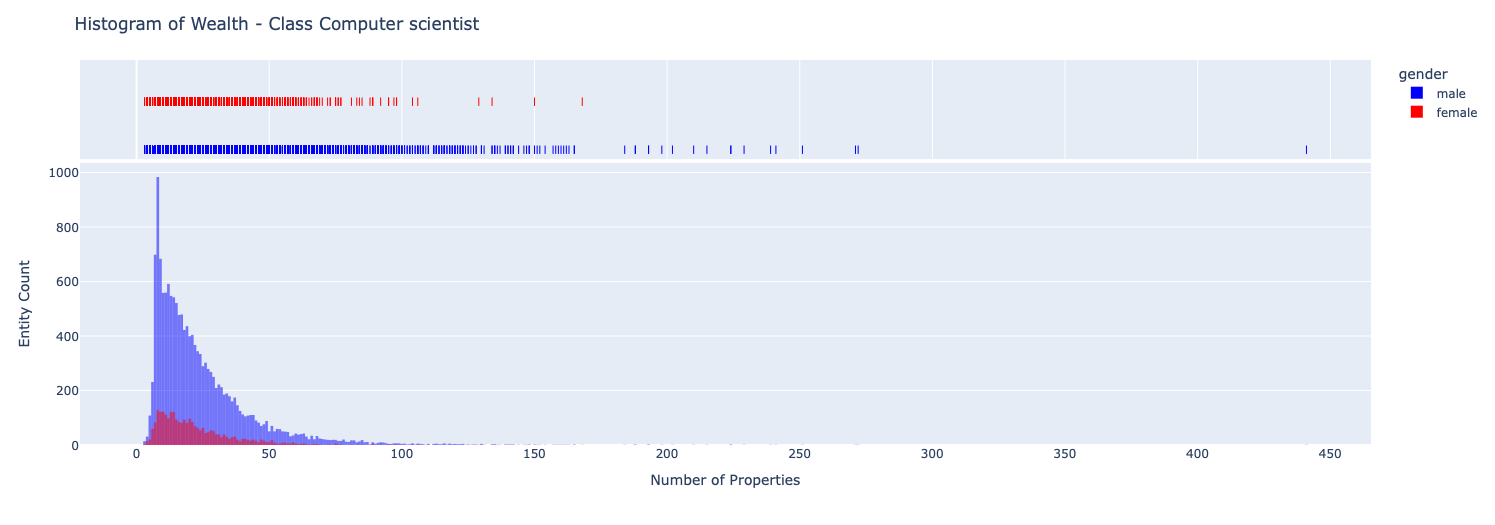
\includegraphics[clip,width=1.0\columnwidth]{Histogram of Wealth - Computer Scientist}%
}

\subfloat[Histogram and Marginal Distribution Plot of Wealth for Class American Singer\label{fig:bias histogram-american singer}]{%
  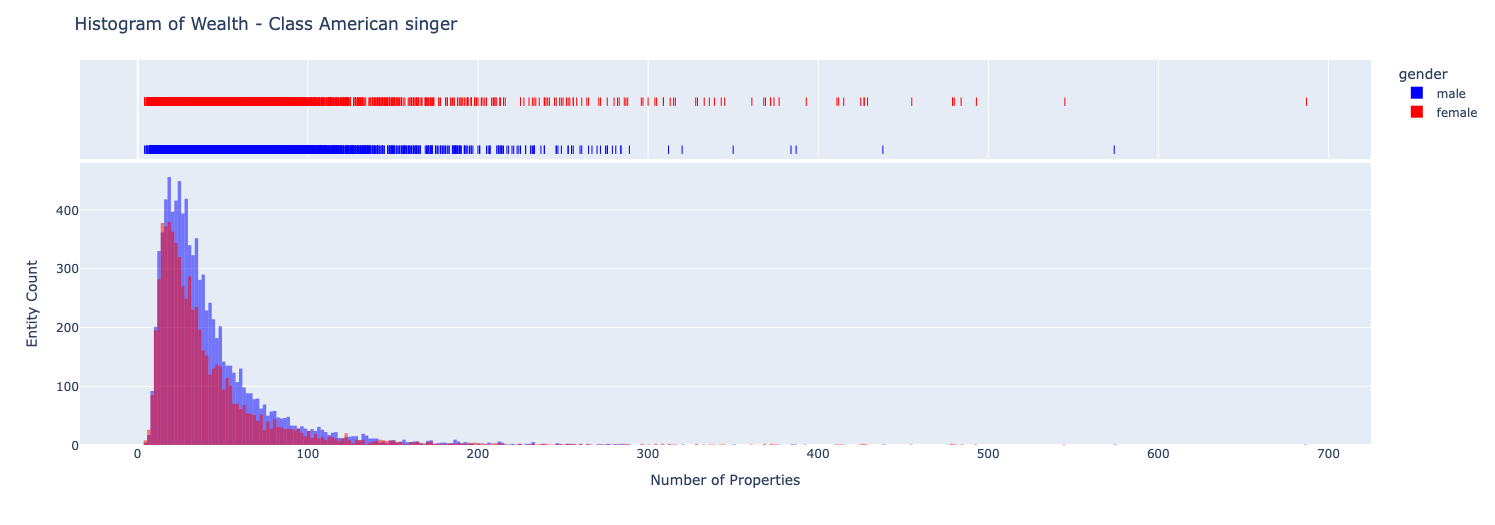
\includegraphics[clip,width=1.0\columnwidth]{Histogram of Wealth - American Singer}%
}

\caption{...}
\label{fig:Histogram of Wealth}

\end{figure}

At a glance we saw female classes are poorer compared to the male classes. To test this, we will use t-test and Welch's test. First, we performed F-test to check if the male and female classes have equal variance. The result of F-test is then used to determine the appropiate test to be used in each class. Those with equal variance will use t-test; otherwise Welch's test is used. Then, we performed the tests to verify the null and alternative hypotheses with significance level of \(\alpha=5\%\) as follows:

\(H_0\): The means of wealth of males and females in a particular class are equal

\(H_1\): The means of wealth of males and females in a particular class are not equal

\begin{center}
\small
\begin{threeparttable}
\caption{F-Test, T-Test, and Welch's Test Result of 10 Wikidata Classes}
\label{tab:gender - mean test}
\begin{tabular}{c c c c c c c} 

\toprule
    Class Name & \CellWithForceBreak{F-Test \\ statistic} & \CellWithForceBreak{F-Test \\ p-value} & \CellWithForceBreak{T-Test \\ statistic} & \CellWithForceBreak{T-Test \\ p-value} & \CellWithForceBreak{Welch's Test \\ statistic} & \CellWithForceBreak{Welch's \\ p-value} \\ [0.5ex] 

\midrule
    American actress/actor & 0.86 & 0.00 & 5.85 & 4.97e-09 & 5.80 & 6.89e-09\\
    American journalist & 1.47 & 1.00 & 12.80 & 2.45e-37 & 13.75 & 1.01e-42 \\
    American politician & 1.00 & 0.55 & 6.86 & 6.90e-12 & 6.87 & 6.94e-12 \\
    American researcher & 1.91 & 1.00 & 6.43 & 1.35e-10 & 7.28 & 4.15e-13 \\
    American singer & 0.64 & 0.00 & 0.75 & 0.45 & 0.73 & 0.47 \\
    American writer & 1.73 & 1.00 & 24.80 & 1.56e-134 & 25.98 & 2.96e-147 \\
    Computer scientist & 1.75 & 1.00 & 5.43 & 5.57e-08 & 6.60 & 4.61e-11 \\
    Badminton player & 0.81 & 0.00 & -2.63 & 8.46e-03 & -2.62 & 8.86e-03 \\
    Businessperson & 0.53 & 0.00 & -4.48 & 7.56e-06 & -3.49 & 4.81e-04 \\
    Lawyer & 1.58 & 1.00 & 27.06 & 1.16e-160 & 32.16 & 8.04e-220 \\
    [1ex]

\bottomrule

\end{tabular}
\begin{tablenotes}
    \footnotesize
    
\end{tablenotes}
\end{threeparttable}
\end{center}

From the test results in \autoref{tab:gender - mean test}, we rejected the null hypothesis in 9 out of 10 class--American singer being the only exception. 7 out of 9 classes are in favor of male. The other 2 classes, American singer and . We concluded that female classes are more likely to have smaller means than male classes.

Here, a new measure is defined: top \(x\)\% male/female relative to the expectation. The value of expectation of a gender in a class is equal to the percentage of that particular in the class. Top \(x\)\% male relative to expectation is the ratio of percentage of male entities in the top \(x\)\% to the expectation. Similarly, top \(x\)\% female relative to expectation is the ratio of percentage of female entities in the top \(x\)\% to the expectation.

When the shape of distribution of male and female of a class is the same (in other word, the wealth is distributed equivalently to male and female entities), then the value of top \(x\)\% relative to expectation should be 1 for both male and female subclasses. A value higher than 1 indicates domination by that particular gender.

\begin{figure}[htp]
\centering 
\subfloat[Ratio of Class Wealth to Expectation per Cumulative Top Percentage - All Classes Average
\label{fig:test1}]{%
  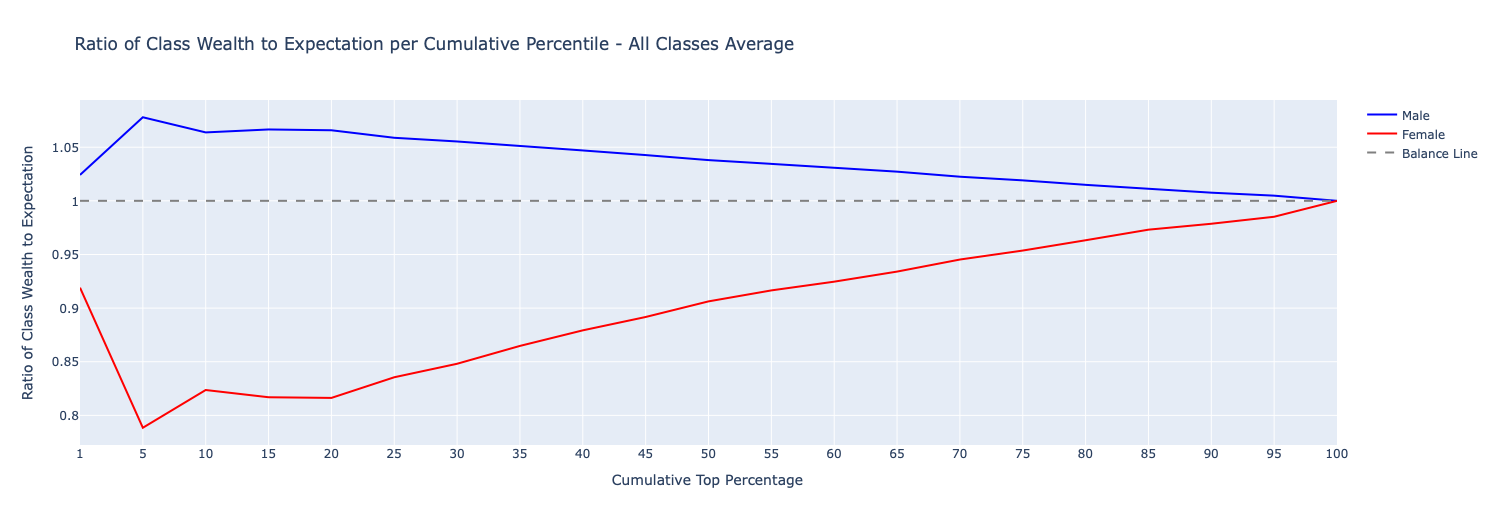
\includegraphics[clip,width=1.0\columnwidth]{Ratio of Class Wealth to Expectation per Cumulative Top Percentage - All Classes Average - Gender}%
}

\subfloat[Ratio of Class Wealth to Expectation per Quantile - All Classes Average\label{fig:test2}]{%
  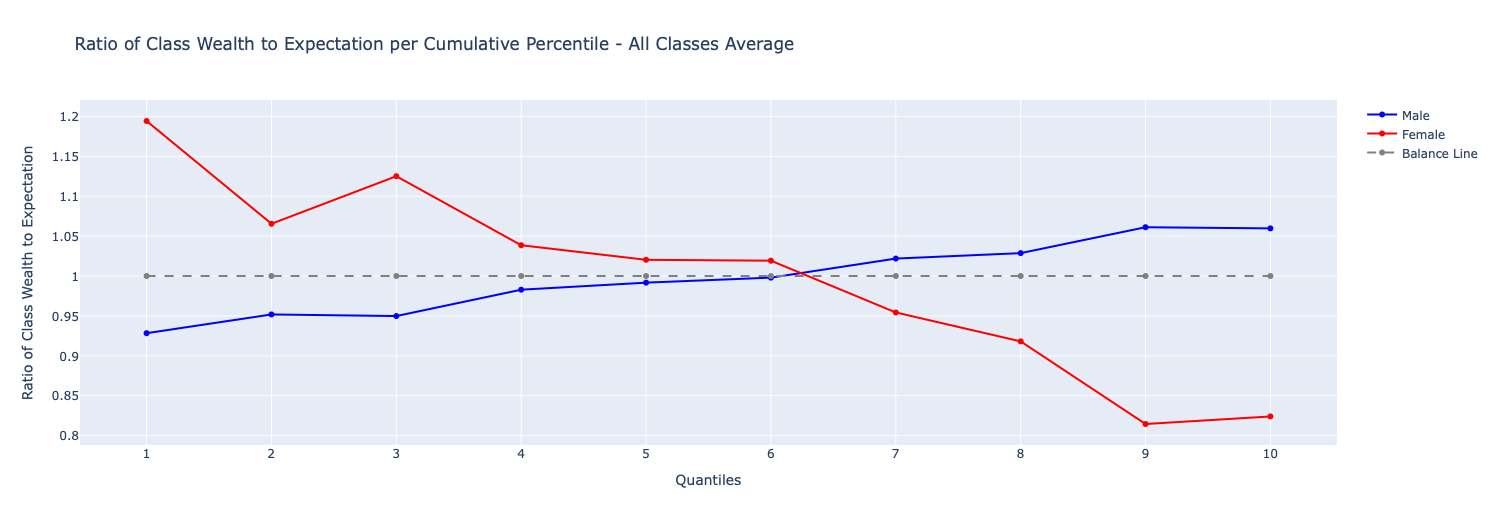
\includegraphics[clip,width=1.0\columnwidth]{Ratio of Class Wealth to Expectation per Quantile - All Classes Average - Gender}%
}

\caption{...}
\label{fig:gender - ratio of gender wealth to expectation}

\end{figure}

From \autoref{fig:gender - ratio of gender wealth to expectation} the value of ratio between top \(x\)\% potion to the expectation in the above tables, we can see that on average, the rich entities are dominated by male. Exceptions are held for 3 classes, that is classes American singer, businessperson, and badminton player. Moreover, as we set bigger portions (higher percentage), the gap of ratio between the two ender in each class decreases i.e. the value of top \(x\)\% relative to expectation of both genders converge to 1.